% Created by tikzDevice version 0.12.6 on 2024-03-12 19:53:23
% !TEX encoding = UTF-8 Unicode
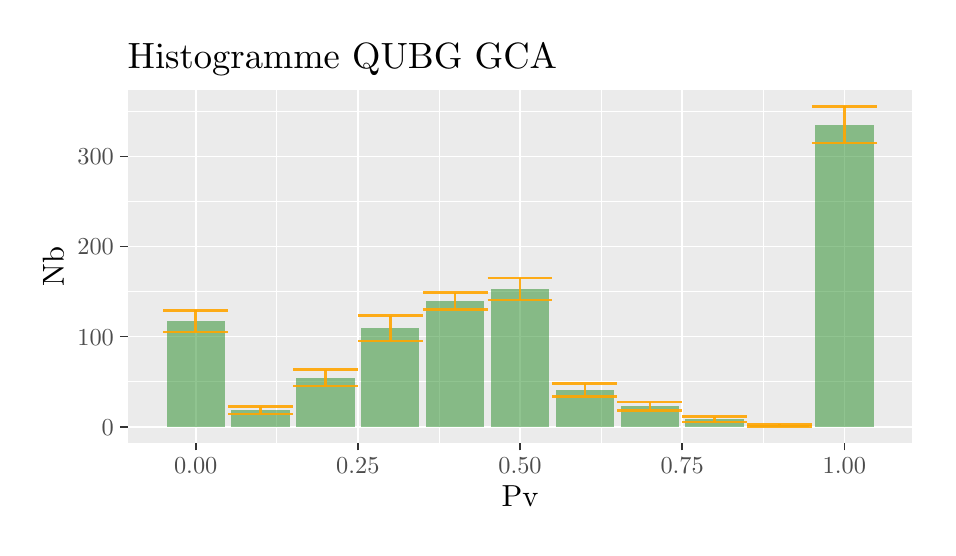
\begin{tikzpicture}[x=1pt,y=1pt]
\definecolor{fillColor}{RGB}{255,255,255}
\path[use as bounding box,fill=fillColor,fill opacity=0.00] (0,0) rectangle (325.21,180.67);
\begin{scope}
\path[clip] (  0.00,  0.00) rectangle (325.21,180.67);
\definecolor{drawColor}{RGB}{255,255,255}
\definecolor{fillColor}{RGB}{255,255,255}

\path[draw=drawColor,line width= 0.6pt,line join=round,line cap=round,fill=fillColor] (  0.00,  0.00) rectangle (325.21,180.68);
\end{scope}
\begin{scope}
\path[clip] ( 36.11, 30.69) rectangle (319.71,158.02);
\definecolor{fillColor}{gray}{0.92}

\path[fill=fillColor] ( 36.11, 30.69) rectangle (319.71,158.02);
\definecolor{drawColor}{RGB}{255,255,255}

\path[draw=drawColor,line width= 0.3pt,line join=round] ( 36.11, 52.75) --
	(319.71, 52.75);

\path[draw=drawColor,line width= 0.3pt,line join=round] ( 36.11, 85.30) --
	(319.71, 85.30);

\path[draw=drawColor,line width= 0.3pt,line join=round] ( 36.11,117.85) --
	(319.71,117.85);

\path[draw=drawColor,line width= 0.3pt,line join=round] ( 36.11,150.40) --
	(319.71,150.40);

\path[draw=drawColor,line width= 0.3pt,line join=round] ( 90.02, 30.69) --
	( 90.02,158.02);

\path[draw=drawColor,line width= 0.3pt,line join=round] (148.62, 30.69) --
	(148.62,158.02);

\path[draw=drawColor,line width= 0.3pt,line join=round] (207.21, 30.69) --
	(207.21,158.02);

\path[draw=drawColor,line width= 0.3pt,line join=round] (265.81, 30.69) --
	(265.81,158.02);

\path[draw=drawColor,line width= 0.6pt,line join=round] ( 36.11, 36.47) --
	(319.71, 36.47);

\path[draw=drawColor,line width= 0.6pt,line join=round] ( 36.11, 69.03) --
	(319.71, 69.03);

\path[draw=drawColor,line width= 0.6pt,line join=round] ( 36.11,101.58) --
	(319.71,101.58);

\path[draw=drawColor,line width= 0.6pt,line join=round] ( 36.11,134.13) --
	(319.71,134.13);

\path[draw=drawColor,line width= 0.6pt,line join=round] ( 60.72, 30.69) --
	( 60.72,158.02);

\path[draw=drawColor,line width= 0.6pt,line join=round] (119.32, 30.69) --
	(119.32,158.02);

\path[draw=drawColor,line width= 0.6pt,line join=round] (177.91, 30.69) --
	(177.91,158.02);

\path[draw=drawColor,line width= 0.6pt,line join=round] (236.51, 30.69) --
	(236.51,158.02);

\path[draw=drawColor,line width= 0.6pt,line join=round] (295.10, 30.69) --
	(295.10,158.02);
\definecolor{fillColor}{RGB}{34,139,34}

\path[fill=fillColor,fill opacity=0.50] ( 50.17, 36.47) rectangle ( 71.27, 74.63);

\path[fill=fillColor,fill opacity=0.50] ( 73.61, 36.47) rectangle ( 94.71, 42.42);

\path[fill=fillColor,fill opacity=0.50] ( 97.05, 36.47) rectangle (118.15, 54.15);

\path[fill=fillColor,fill opacity=0.50] (120.49, 36.47) rectangle (141.58, 72.04);

\path[fill=fillColor,fill opacity=0.50] (143.93, 36.47) rectangle (165.02, 81.87);

\path[fill=fillColor,fill opacity=0.50] (167.37, 36.47) rectangle (188.46, 86.26);

\path[fill=fillColor,fill opacity=0.50] (190.80, 36.47) rectangle (211.90, 49.78);

\path[fill=fillColor,fill opacity=0.50] (214.24, 36.47) rectangle (235.34, 43.84);

\path[fill=fillColor,fill opacity=0.50] (237.68, 36.47) rectangle (258.78, 39.16);

\path[fill=fillColor,fill opacity=0.50] (261.12, 36.47) rectangle (282.21, 36.95);

\path[fill=fillColor,fill opacity=0.50] (284.56, 36.47) rectangle (305.65,145.63);
\definecolor{drawColor}{RGB}{255,165,0}

\path[draw=drawColor,draw opacity=0.90,line width= 0.9pt,line join=round] ( 49.00, 78.49) --
	( 72.44, 78.49);

\path[draw=drawColor,draw opacity=0.90,line width= 0.9pt,line join=round] ( 60.72, 78.49) --
	( 60.72, 70.77);

\path[draw=drawColor,draw opacity=0.90,line width= 0.9pt,line join=round] ( 49.00, 70.77) --
	( 72.44, 70.77);

\path[draw=drawColor,draw opacity=0.90,line width= 0.9pt,line join=round] ( 72.44, 43.75) --
	( 95.88, 43.75);

\path[draw=drawColor,draw opacity=0.90,line width= 0.9pt,line join=round] ( 84.16, 43.75) --
	( 84.16, 41.09);

\path[draw=drawColor,draw opacity=0.90,line width= 0.9pt,line join=round] ( 72.44, 41.09) --
	( 95.88, 41.09);

\path[draw=drawColor,draw opacity=0.90,line width= 0.9pt,line join=round] ( 95.88, 57.14) --
	(119.32, 57.14);

\path[draw=drawColor,draw opacity=0.90,line width= 0.9pt,line join=round] (107.60, 57.14) --
	(107.60, 51.16);

\path[draw=drawColor,draw opacity=0.90,line width= 0.9pt,line join=round] ( 95.88, 51.16) --
	(119.32, 51.16);

\path[draw=drawColor,draw opacity=0.90,line width= 0.9pt,line join=round] (119.32, 76.65) --
	(142.76, 76.65);

\path[draw=drawColor,draw opacity=0.90,line width= 0.9pt,line join=round] (131.04, 76.65) --
	(131.04, 67.42);

\path[draw=drawColor,draw opacity=0.90,line width= 0.9pt,line join=round] (119.32, 67.42) --
	(142.76, 67.42);

\path[draw=drawColor,draw opacity=0.90,line width= 0.9pt,line join=round] (142.76, 84.91) --
	(166.19, 84.91);

\path[draw=drawColor,draw opacity=0.90,line width= 0.9pt,line join=round] (154.47, 84.91) --
	(154.47, 78.83);

\path[draw=drawColor,draw opacity=0.90,line width= 0.9pt,line join=round] (142.76, 78.83) --
	(166.19, 78.83);

\path[draw=drawColor,draw opacity=0.90,line width= 0.9pt,line join=round] (166.19, 90.26) --
	(189.63, 90.26);

\path[draw=drawColor,draw opacity=0.90,line width= 0.9pt,line join=round] (177.91, 90.26) --
	(177.91, 82.26);

\path[draw=drawColor,draw opacity=0.90,line width= 0.9pt,line join=round] (166.19, 82.26) --
	(189.63, 82.26);

\path[draw=drawColor,draw opacity=0.90,line width= 0.9pt,line join=round] (189.63, 52.08) --
	(213.07, 52.08);

\path[draw=drawColor,draw opacity=0.90,line width= 0.9pt,line join=round] (201.35, 52.08) --
	(201.35, 47.48);

\path[draw=drawColor,draw opacity=0.90,line width= 0.9pt,line join=round] (189.63, 47.48) --
	(213.07, 47.48);

\path[draw=drawColor,draw opacity=0.90,line width= 0.9pt,line join=round] (213.07, 45.40) --
	(236.51, 45.40);

\path[draw=drawColor,draw opacity=0.90,line width= 0.9pt,line join=round] (224.79, 45.40) --
	(224.79, 42.27);

\path[draw=drawColor,draw opacity=0.90,line width= 0.9pt,line join=round] (213.07, 42.27) --
	(236.51, 42.27);

\path[draw=drawColor,draw opacity=0.90,line width= 0.9pt,line join=round] (236.51, 40.13) --
	(259.95, 40.13);

\path[draw=drawColor,draw opacity=0.90,line width= 0.9pt,line join=round] (248.23, 40.13) --
	(248.23, 38.20);

\path[draw=drawColor,draw opacity=0.90,line width= 0.9pt,line join=round] (236.51, 38.20) --
	(259.95, 38.20);

\path[draw=drawColor,draw opacity=0.90,line width= 0.9pt,line join=round] (259.95, 37.33) --
	(283.39, 37.33);

\path[draw=drawColor,draw opacity=0.90,line width= 0.9pt,line join=round] (271.67, 37.33) --
	(271.67, 36.58);

\path[draw=drawColor,draw opacity=0.90,line width= 0.9pt,line join=round] (259.95, 36.58) --
	(283.39, 36.58);

\path[draw=drawColor,draw opacity=0.90,line width= 0.9pt,line join=round] (283.39,152.23) --
	(306.82,152.23);

\path[draw=drawColor,draw opacity=0.90,line width= 0.9pt,line join=round] (295.10,152.23) --
	(295.10,139.03);

\path[draw=drawColor,draw opacity=0.90,line width= 0.9pt,line join=round] (283.39,139.03) --
	(306.82,139.03);
\end{scope}
\begin{scope}
\path[clip] (  0.00,  0.00) rectangle (325.21,180.67);
\definecolor{drawColor}{gray}{0.30}

\node[text=drawColor,anchor=base east,inner sep=0pt, outer sep=0pt, scale=  0.88] at ( 31.16, 33.44) {0};

\node[text=drawColor,anchor=base east,inner sep=0pt, outer sep=0pt, scale=  0.88] at ( 31.16, 65.99) {100};

\node[text=drawColor,anchor=base east,inner sep=0pt, outer sep=0pt, scale=  0.88] at ( 31.16, 98.55) {200};

\node[text=drawColor,anchor=base east,inner sep=0pt, outer sep=0pt, scale=  0.88] at ( 31.16,131.10) {300};
\end{scope}
\begin{scope}
\path[clip] (  0.00,  0.00) rectangle (325.21,180.67);
\definecolor{drawColor}{gray}{0.20}

\path[draw=drawColor,line width= 0.6pt,line join=round] ( 33.36, 36.47) --
	( 36.11, 36.47);

\path[draw=drawColor,line width= 0.6pt,line join=round] ( 33.36, 69.03) --
	( 36.11, 69.03);

\path[draw=drawColor,line width= 0.6pt,line join=round] ( 33.36,101.58) --
	( 36.11,101.58);

\path[draw=drawColor,line width= 0.6pt,line join=round] ( 33.36,134.13) --
	( 36.11,134.13);
\end{scope}
\begin{scope}
\path[clip] (  0.00,  0.00) rectangle (325.21,180.67);
\definecolor{drawColor}{gray}{0.20}

\path[draw=drawColor,line width= 0.6pt,line join=round] ( 60.72, 27.94) --
	( 60.72, 30.69);

\path[draw=drawColor,line width= 0.6pt,line join=round] (119.32, 27.94) --
	(119.32, 30.69);

\path[draw=drawColor,line width= 0.6pt,line join=round] (177.91, 27.94) --
	(177.91, 30.69);

\path[draw=drawColor,line width= 0.6pt,line join=round] (236.51, 27.94) --
	(236.51, 30.69);

\path[draw=drawColor,line width= 0.6pt,line join=round] (295.10, 27.94) --
	(295.10, 30.69);
\end{scope}
\begin{scope}
\path[clip] (  0.00,  0.00) rectangle (325.21,180.67);
\definecolor{drawColor}{gray}{0.30}

\node[text=drawColor,anchor=base,inner sep=0pt, outer sep=0pt, scale=  0.88] at ( 60.72, 19.68) {0.00};

\node[text=drawColor,anchor=base,inner sep=0pt, outer sep=0pt, scale=  0.88] at (119.32, 19.68) {0.25};

\node[text=drawColor,anchor=base,inner sep=0pt, outer sep=0pt, scale=  0.88] at (177.91, 19.68) {0.50};

\node[text=drawColor,anchor=base,inner sep=0pt, outer sep=0pt, scale=  0.88] at (236.51, 19.68) {0.75};

\node[text=drawColor,anchor=base,inner sep=0pt, outer sep=0pt, scale=  0.88] at (295.10, 19.68) {1.00};
\end{scope}
\begin{scope}
\path[clip] (  0.00,  0.00) rectangle (325.21,180.67);
\definecolor{drawColor}{RGB}{0,0,0}

\node[text=drawColor,anchor=base,inner sep=0pt, outer sep=0pt, scale=  1.10] at (177.91,  7.64) {Pv};
\end{scope}
\begin{scope}
\path[clip] (  0.00,  0.00) rectangle (325.21,180.67);
\definecolor{drawColor}{RGB}{0,0,0}

\node[text=drawColor,rotate= 90.00,anchor=base,inner sep=0pt, outer sep=0pt, scale=  1.10] at ( 13.08, 94.35) {Nb};
\end{scope}
\begin{scope}
\path[clip] (  0.00,  0.00) rectangle (325.21,180.67);
\definecolor{drawColor}{RGB}{0,0,0}

\node[text=drawColor,anchor=base west,inner sep=0pt, outer sep=0pt, scale=  1.32] at ( 36.11,166.08) {Histogramme QUBG GCA};
\end{scope}
\end{tikzpicture}
